\documentclass[conference]{IEEEtran}
\usepackage[utf8]{inputenc}
\usepackage[T1]{fontenc}
\usepackage[spanish,es-tabla,es-nodecimaldot,es-noshorthands]{babel}
\usepackage{amsmath,amssymb}
\usepackage{graphicx}
\usepackage{booktabs}
\usepackage{array}
\usepackage{adjustbox}
\usepackage{tikz}
\usetikzlibrary{arrows.meta,positioning}
\usepackage{url}
\usepackage[hidelinks]{hyperref}

\graphicspath{{../results/figures/}}
% Several page-wide tables per page; the default (1) pushes them pages behind their text.
\setcounter{dbltopnumber}{4}
\renewcommand{\dbltopfraction}{0.95}
\renewcommand{\dblfloatpagefraction}{0.8}
\renewcommand{\topfraction}{0.9}
\renewcommand{\textfraction}{0.1}
\renewcommand{\IEEEkeywordsname}{Palabras clave}
% Line break between author rows (IEEEtran puts 3 per row; 2x2 keeps the 4 authors centered).
\makeatletter
\newcommand{\linebreakand}{\end{@IEEEauthorhalign}\hfill\mbox{}\par\mbox{}\hfill\begin{@IEEEauthorhalign}}
\makeatother
\newcommand{\tab}[1]{\input{../results/tables/#1.tex}}
\newcommand{\pc}{p_{\mathrm{c\acute{a}ncer}}}

\begin{document}

\title{Triaje de cáncer de piel en fotos de smartphone con augmentation de adquisición: CNN frente a Vision Transformer}

\author{\IEEEauthorblockN{Juan Burgos Choquehuanca}
\IEEEauthorblockA{Maestría en Inteligencia Artificial\\
FIIS -- UNI\\
Lima, Perú\\
juan.burgos.c@uni.pe}
\and
\IEEEauthorblockN{David Roberto Paredes Abanto}
\IEEEauthorblockA{Maestría en Inteligencia Artificial\\
FIIS -- UNI\\
Lima, Perú\\
david.paredes.a@uni.pe}
\linebreakand
\IEEEauthorblockN{Carlos Adrian Salguero Torres}
\IEEEauthorblockA{Maestría en Inteligencia Artificial\\
FIIS -- UNI\\
Lima, Perú\\
carlos.salguero.t@uni.pe}
\and
\IEEEauthorblockN{Huber Angel Ramirez Quispe}
\IEEEauthorblockA{Maestría en Inteligencia Artificial\\
FIIS -- UNI\\
Lima, Perú\\
huber.ramirez.q@uni.pe}}

\maketitle

\begin{abstract}
Las fotos de lesiones cutáneas tomadas con un smartphone en atención primaria llegan con mala iluminación, desenfoque, ruido, compresión o vello, y los clasificadores entrenados con imágenes limpias pierden precisión justo donde un error de triaje es más costoso. Estudiamos el triaje cáncer (carcinoma basocelular, melanoma y carcinoma espinocelular) frente a no cáncer en PAD-UFES-20, con partición por paciente. Ajustamos finamente EfficientNet-B0 y ViT-S/16 sin augmentation, con augmentation geométrica estándar y con una augmentation de adquisición que simula esas degradaciones, y medimos la robustez con 6 corrupciones a 5 severidades, dos de ellas nunca vistas en entrenamiento. ViT-S/16 alcanza una AUC de 0.930 y una especificidad de 0.81--0.83 a sensibilidad 90\,\%, frente a 0.825 y 0.445 de una línea base ResNet-50 congelada con regresión logística. La augmentation de adquisición reduce la caída relativa de AUC de EfficientNet-B0 bajo corrupción del 22.5\,\% al 2.7\,\% en las corrupciones vistas y del 20.1\,\% al 4.8\,\% en las no vistas, sin perder AUC en imágenes limpias; ViT-S/16 cae solo un 4.2\,\% sin augmentation y un 1.6--2.0\,\% con ella. Un modelo entrenado con imágenes dermatoscópicas (HAM10000) pierde 0.143 de AUC en estas fotos. Concluimos que un sistema de triaje con fotos de smartphone debe entrenarse con degradaciones realistas o con una arquitectura robusta, y validarse con pruebas de estrés antes de su uso.
\end{abstract}

\begin{IEEEkeywords}
aprendizaje profundo, cáncer de piel, triaje, robustez, augmentation de datos, vision transformer
\end{IEEEkeywords}

% ---------------------------------------------------------------------------
\section{Introducción}

El cáncer de piel es uno de los cánceres más frecuentes y su pronóstico depende de detectarlo a tiempo, pero el acceso a dermatología es limitado fuera de las grandes ciudades. Un smartphone en manos de un médico de atención primaria puede servir para decidir qué lesiones derivar al especialista. El aprendizaje profundo ya alcanza un desempeño comparable al de dermatólogos con imágenes cuidadas \cite{esteva2017}, pero las aplicaciones de smartphone para evaluar riesgo de cáncer de piel tienen evidencia de exactitud limitada y poco fiable \cite{freeman2020}, y los modelos dermatológicos cambian su predicción ante transformaciones simples de la imagen \cite{young2021,maron2021}. Las fotos reales llegan con la luz disponible, tomadas a pulso, comprimidas y a veces con vello sobre la lesión.

\textbf{Formulación.} La entrada es una foto clínica de una lesión tomada con smartphone. La salida es la probabilidad de cáncer $\pc$ y la decisión de derivar cuando $\pc$ supera un umbral. Definimos cáncer como carcinoma basocelular (BCC), melanoma (MEL) y carcinoma espinocelular (SCC), frente a queratosis actínica (ACK), nevo (NEV) y queratosis seborreica (SEK). El éxito se mide con la AUC cáncer frente a no cáncer y con la especificidad a sensibilidad 90\,\%, y debe mantenerse cuando la foto se degrada.

\textbf{Enfoque.} Usamos aprendizaje profundo porque los rasgos que distinguen una lesión maligna (bordes, color, textura) son difíciles de describir a mano y las redes preentrenadas en ImageNet los aprenden con pocos miles de imágenes. Comparamos dos arquitecturas con supuestos distintos: EfficientNet-B0 \cite{tan2019}, una CNN eficiente cuyos filtros locales aprovechan la textura, y ViT-S/16 \cite{dosovitskiy2021}, un Transformer \cite{vaswani2017} que relaciona todos los parches de la imagen desde la primera capa. Ambos tienen un costo de inferencia similar. La idea principal es una augmentation de adquisición que expone al modelo, durante el entrenamiento, a las degradaciones que encontrará en uso, evaluada con corrupciones vistas y no vistas para que la mejora no sea circular. Contrastamos tres hipótesis: \textbf{H1}, la augmentation de adquisición reduce la caída bajo corrupción frente a la augmentation estándar, también en corrupciones no vistas; \textbf{H2}, el ViT se degrada distinto que la CNN; y \textbf{H3}, un modelo entrenado con imágenes dermatoscópicas pierde desempeño en fotos de smartphone.

Las contribuciones de este trabajo son:
\begin{itemize}
\item Un banco de 6 corrupciones de adquisición deterministas a 5 severidades, dos de ellas reservadas solo para la evaluación.
\item Una augmentation de adquisición para el entrenamiento y su comparación entre una CNN y un Vision Transformer, con la misma partición por paciente y las mismas corrupciones.
\item Una evaluación con 3 semillas, umbral de operación fijado en validación, diferencias emparejadas por bootstrap de pacientes, un experimento de transferencia desde imágenes dermatoscópicas, y análisis por subtipo, por fototipo y de mapas de atención, en un repositorio que regenera cada número con un comando.
\end{itemize}

El resto del artículo se organiza así: la Sección~\ref{sec:related} revisa trabajos relacionados; la Sección~\ref{sec:method} describe la metodología; la Sección~\ref{sec:results} presenta los resultados, que se discuten en la Sección~\ref{sec:discussion}; la Sección~\ref{sec:conclusions} concluye.

% ---------------------------------------------------------------------------
\section{Trabajos relacionados}
\label{sec:related}

\textbf{Clasificación de lesiones cutáneas.} Esteva et al.\ \cite{esteva2017} entrenaron una CNN con unas 130\,000 imágenes clínicas y obtuvieron un desempeño de nivel dermatólogo. HAM10000 \cite{tschandl2018} reúne 10\,015 imágenes dermatoscópicas de 7 diagnósticos y es una referencia habitual. PAD-UFES-20 \cite{pacheco2020pad} es, en cambio, un conjunto de fotos clínicas de smartphone con metadatos del paciente; sobre él, Pacheco y Krohling \cite{pacheco2021metablock} combinan imagen y metadatos clínicos con un mecanismo de atención y reportan una BACC en 6 clases cercana a 0.77 con validación cruzada. Nosotros usamos solo la imagen, porque nuestro foco es la robustez a la calidad de la foto, y reportamos el triaje binario que corresponde a la decisión de derivar.

\textbf{Arquitecturas.} ResNet \cite{he2016} introdujo las conexiones residuales que permiten entrenar CNN profundas, y EfficientNet \cite{tan2019} escala profundidad, ancho y resolución de forma conjunta para obtener redes eficientes. El Transformer \cite{vaswani2017} reemplaza la recurrencia por autoatención, y ViT \cite{dosovitskiy2021} lo aplica a secuencias de parches de imagen. Partimos de pesos de ImageNet \cite{deng2009} vía \texttt{timm} \cite{wightman2019}. Bhojanapalli et al.\ \cite{bhojanapalli2021} encontraron que los ViT son tan o más robustos que las CNN ante perturbaciones naturales; nosotros lo verificamos en fotos clínicas y medimos cuánto de esa ventaja se recupera en la CNN con augmentation.

\textbf{Robustez y atajos en dermatología.} Hendrycks y Dietterich \cite{hendrycks2019} propusieron medir la robustez con corrupciones comunes a varias severidades. Maron et al.\ \cite{maron2021} construyeron un banco de corrupciones para imágenes dermatoscópicas y encontraron que las CNN son vulnerables, y Young et al.\ \cite{young2021} mostraron que rotaciones y nuevas capturas de la misma lesión cambian la predicción en una fracción relevante de casos. Winkler et al.\ \cite{winkler2019} mostraron que las marcas de tinta elevan la probabilidad de melanoma de nevos benignos, y Daneshjou et al.\ \cite{daneshjou2022} documentaron caídas de desempeño en fototipos oscuros. A diferencia de \cite{maron2021,young2021}, que evalúan modelos dermatoscópicos ya entrenados, nosotros entrenamos con una augmentation de adquisición en fotos de smartphone y separamos corrupciones vistas y no vistas.

\textbf{Interpretabilidad.} Grad-CAM \cite{selvaraju2017} pondera los mapas de activación de una CNN con el gradiente de la clase, y attention rollout \cite{abnar2020} propaga la atención de un Transformer a través de las capas. Darcet et al.\ \cite{darcet2024} describen tokens de norma alta en los ViT que producen artefactos en estos mapas.

% ---------------------------------------------------------------------------
\section{Metodología}
\label{sec:method}

\subsection{Datos}
PAD-UFES-20 \cite{pacheco2020pad} (licencia CC BY 4.0) contiene 2298 fotos clínicas de 1641 lesiones de 1373 pacientes, tomadas con smartphones en un programa de dermatología de Brasil. Sus 6 clases están desbalanceadas: ACK (730), BCC (845), MEL (52), NEV (244), SCC (192) y SEK (235). Las 1089 imágenes de cáncer y las 1209 de no cáncer dan un triaje casi balanceado. Para evitar la fuga de datos, particionamos por paciente, estratificado por clase, de modo que ningún paciente aparece en dos particiones (Tabla~\ref{tab:data}). Las imágenes se reducen a 256~px en el lado corto y se guardan en PNG, para que la compresión JPEG del banco de corrupciones parta de imágenes sin pérdida.

\tab{data}

\textbf{Augmentation.} Comparamos tres distribuciones de transformaciones $\mathcal{T}$ en entrenamiento:
\begin{itemize}
\item \texttt{none}: redimensionado y recorte central a 224~px.
\item \texttt{standard}: rotación de hasta 90°, recorte aleatorio (60--100\,\% del área) y volteos horizontal y vertical.
\item \texttt{robust}: \texttt{standard} más gamma (0.7--1.5), temperatura de color ($\pm$10\,\%), \textit{color jitter} y, con probabilidad 0.3 cada una, las cuatro corrupciones vistas a una severidad aleatoria de 1 a 5.
\end{itemize}

\textbf{Banco de corrupciones.} Definimos 6 corrupciones con 5 severidades (Fig.~\ref{fig:corr}), aplicadas sobre la imagen de 256~px antes del recorte. Las \emph{vistas}, que también usa \texttt{robust}, son brillo (exposición $\pm$10--50\,\%), desenfoque gaussiano ($\sigma$ de 1 a 6~px), ruido gaussiano ($\sigma$ de 3 a 18\,\% del rango) y vello sintético (3 a 24 curvas oscuras). Las \emph{no vistas}, solo en test, son desenfoque de movimiento (núcleo de 5 a 23~px con ángulo aleatorio) y compresión JPEG (calidad 50 a 10). Separarlas evita una evaluación circular. Cada corrupción es determinista: su generador aleatorio se siembra con la imagen, la corrupción y la severidad.

\textbf{Transferencia (H3).} Usamos HAM10000 \cite{tschandl2018} (10\,015 imágenes dermatoscópicas, licencia CC BY-NC 4.0) con los diagnósticos mapeados a las clases de PAD: \texttt{mel}$\to$MEL, \texttt{bcc}$\to$BCC, \texttt{akiec}$\to$SCC, \texttt{nv}$\to$NEV, \texttt{bkl}$\to$SEK y \texttt{df}, \texttt{vasc}$\to$ACK. Lo particionamos por lesión en entrenamiento y validación (6:1) y evaluamos en el mismo test de PAD.

\subsection{Arquitectura propuesta}
La Fig.~\ref{fig:pipeline} muestra el modelo con las dimensiones de los tensores. La foto se recorta a $3\times224\times224$ y se normaliza con la media y la desviación de ImageNet dentro del modelo. EfficientNet-B0 produce un mapa de $1280\times7\times7$ que se promedia espacialmente; ViT-S/16 divide la imagen en $14\times14=196$ parches de $16\times16$~px, les suma un token de clase y, tras 12 bloques de autoatención, toma el token de clase de dimensión 384. Una capa lineal nueva produce los 6 logits. Los backbones parten de ImageNet y se ajustan completos; solo la cabeza se inicializa al azar. Entrenamos en 6 clases y no en binario porque la supervisión más fina separa subtipos con aspecto distinto (p.\,ej. MEL frente a BCC) y porque una sola corrida da el triaje, la clasificación en 6 clases y la sensibilidad por subtipo. La línea base usa las características congeladas de ResNet-50 \cite{he2016} con una regresión logística con pesos de clase balanceados.

\begin{figure}[t]
\centering
\begin{tikzpicture}[node distance=2.5mm, every node/.style={font=\scriptsize, align=center},
  box/.style={draw, rounded corners, minimum height=8mm, inner sep=2pt}, >=Stealth]
\node[box] (img) {Foto\\$3{\times}224{\times}224$};
\node[box, right=of img] (net) {EfficientNet-B0\\$1280{\times}7{\times}7\to1280$\\[2pt]ViT-S/16\\$197{\times}384\to384$};
\node[box, right=of net] (head) {Lineal\\6 logits};
\node[box, below=4mm of head] (soft) {softmax\\$\pc\geq\tau$?};
\node[box, left=5mm of soft] (out) {derivar /\\no derivar};
\node[box, above=3mm of img, dashed] (aug) {$T\sim\mathcal{T}$\\(solo entrenamiento)};
\draw[->] (img) -- (net); \draw[->] (net) -- (head); \draw[->] (head) -- (soft); \draw[->] (soft) -- (out);
\draw[->, dashed] (aug) -- (img);
\end{tikzpicture}
\caption{Arquitectura. El backbone preentrenado en ImageNet se ajusta completo; la cabeza lineal es nueva. El umbral $\tau$ se fija en validación a sensibilidad 90\,\%.}
\label{fig:pipeline}
\end{figure}

\begin{figure*}[t]
\centering
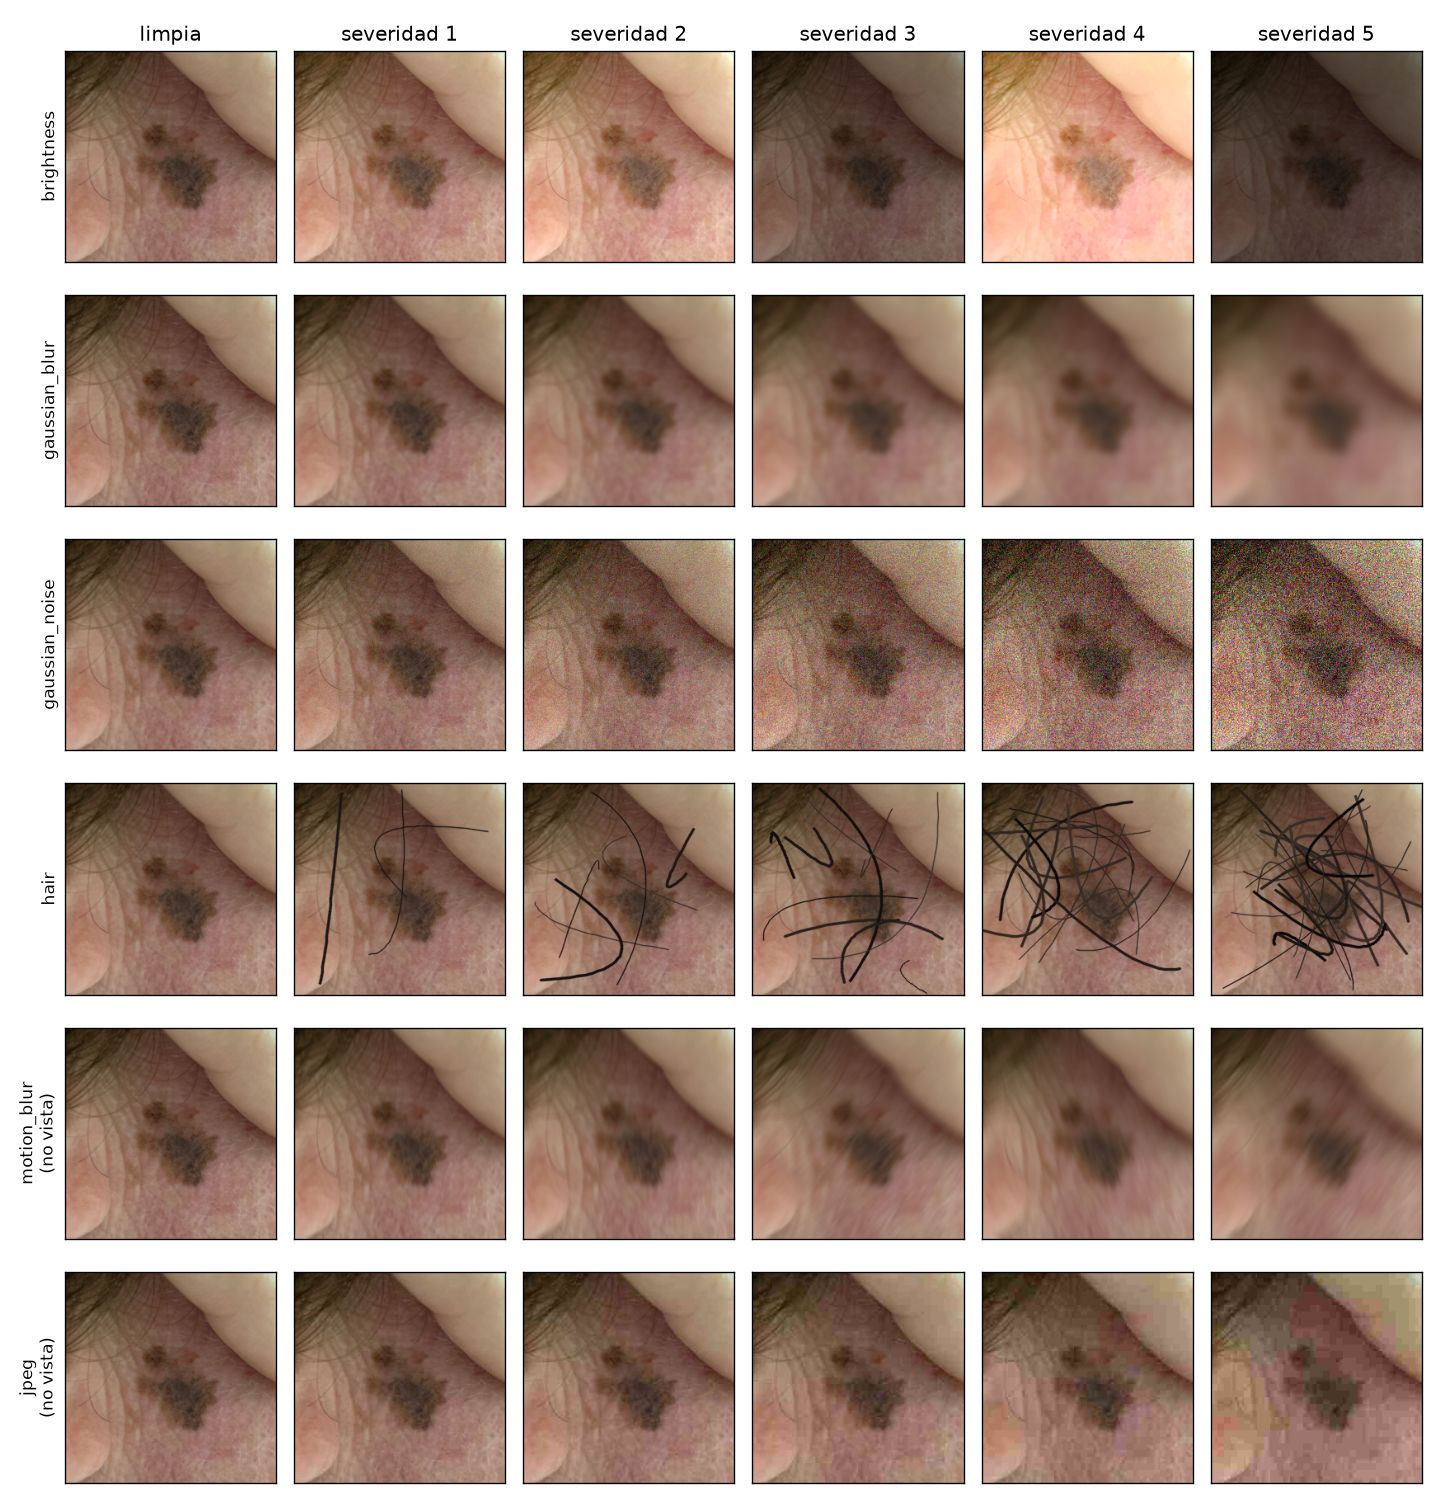
\includegraphics[width=0.9\textwidth]{corruptions_grid.png}
\caption{Las 6 corrupciones de adquisición a severidades 1--5 sobre una imagen de PAD-UFES-20. motion blur y jpeg no se usan en entrenamiento.}
\label{fig:corr}
\end{figure*}

\subsection{Formulación y función de pérdida}
Sea $p_\theta(c\mid x)$ la salida softmax del modelo para la clase $c$. El puntaje de triaje es la probabilidad agregada de cáncer
\begin{equation}
\pc(x) = p_\theta(\mathrm{BCC}\mid x) + p_\theta(\mathrm{MEL}\mid x) + p_\theta(\mathrm{SCC}\mid x),
\end{equation}
y la lesión se deriva si $\pc(x)\geq\tau$. Minimizamos la entropía cruzada ponderada por clase sobre $N$ imágenes y $C=6$ clases,
\begin{equation}
\mathcal{L}(\theta) = -\frac{1}{N}\sum_{i=1}^{N}\sum_{c=1}^{C} w_c\, y_{i,c}\log p_\theta(c\mid T(x_i)),\quad w_c = \frac{N}{C\,n_c},
\end{equation}
donde $y_{i,c}$ es la etiqueta one-hot, $n_c$ el número de imágenes de la clase $c$ en entrenamiento y $T\sim\mathcal{T}$ la transformación de augmentation; en esperanza se minimiza $\mathbb{E}_{(x,y)}\,\mathbb{E}_{T\sim\mathcal{T}}[\ell(f_\theta(T(x)),y)]$. Los pesos $w_c$ compensan el desbalance, en particular los 37 melanomas de entrenamiento.

% Results floats are defined here so they land next to Section IV.
\tab{main}
\tab{main_6class}
\begin{figure*}[t]
\centering
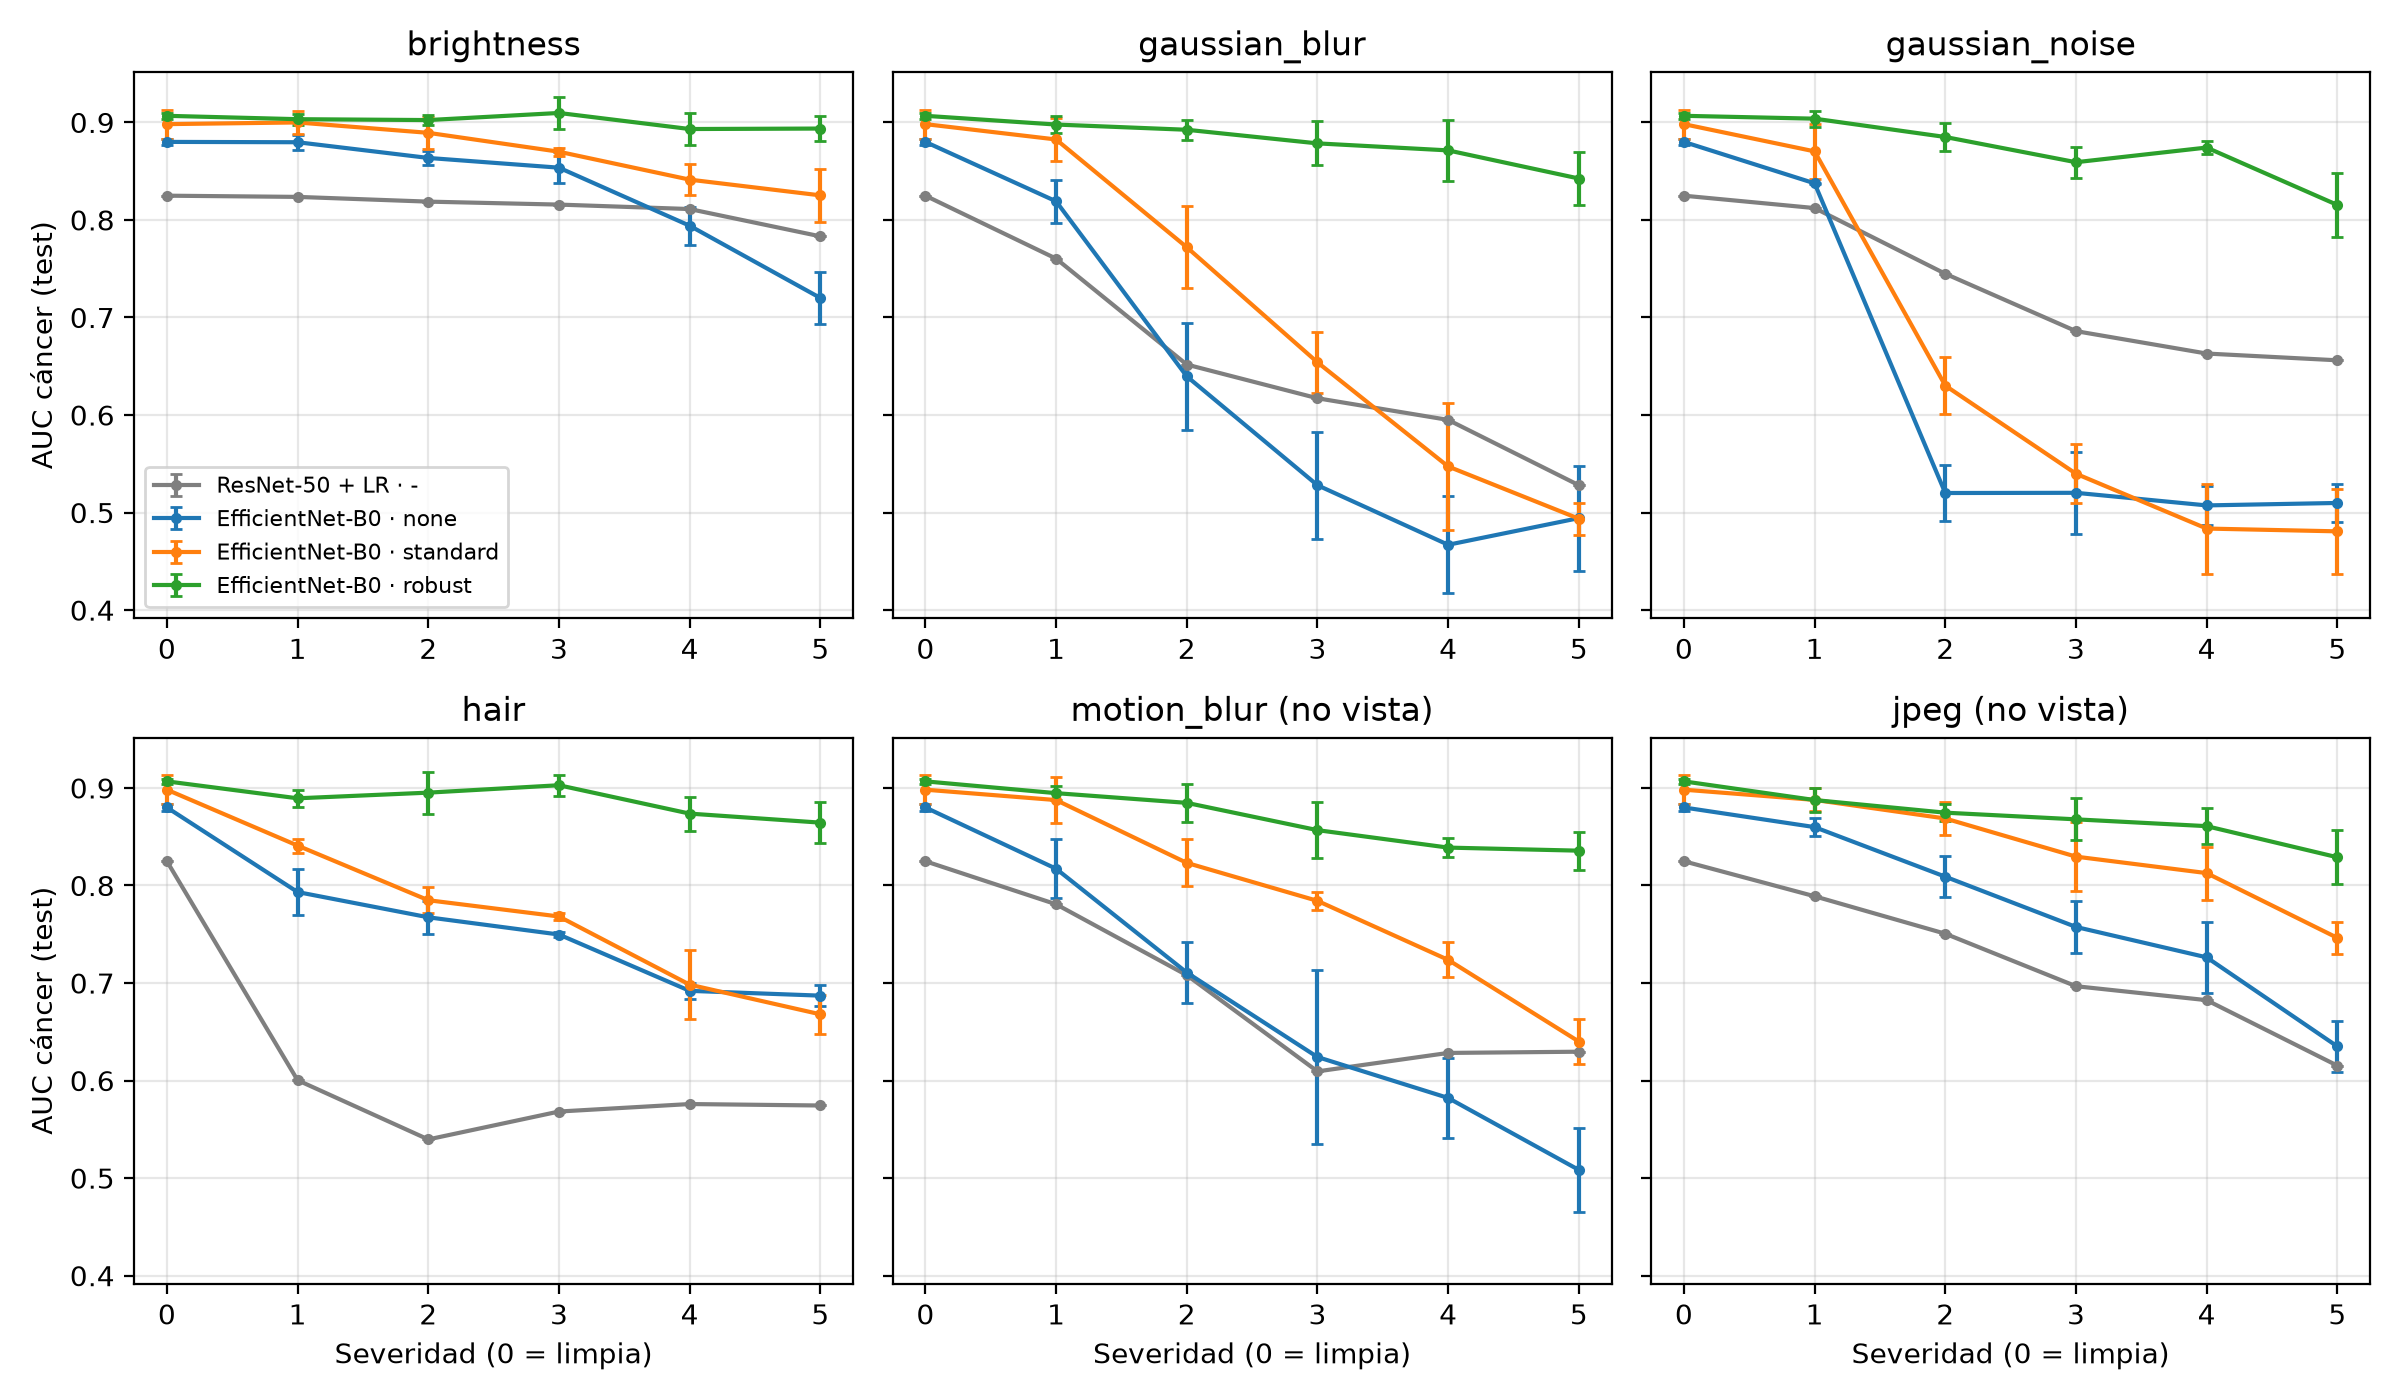
\includegraphics[width=\textwidth]{robustness_curve.png}
\caption{AUC cáncer en test frente a la severidad de cada corrupción (media $\pm$ sd entre semillas). Línea continua: EfficientNet-B0; discontinua: ViT-S/16; punteada: EfficientNet-B0 entrenado en HAM10000; gris: línea base.}
\label{fig:curve}
\end{figure*}
\tab{robustness}
\tab{paired}
\begin{figure*}[t]
\centering
\begin{minipage}{0.49\textwidth}\centering
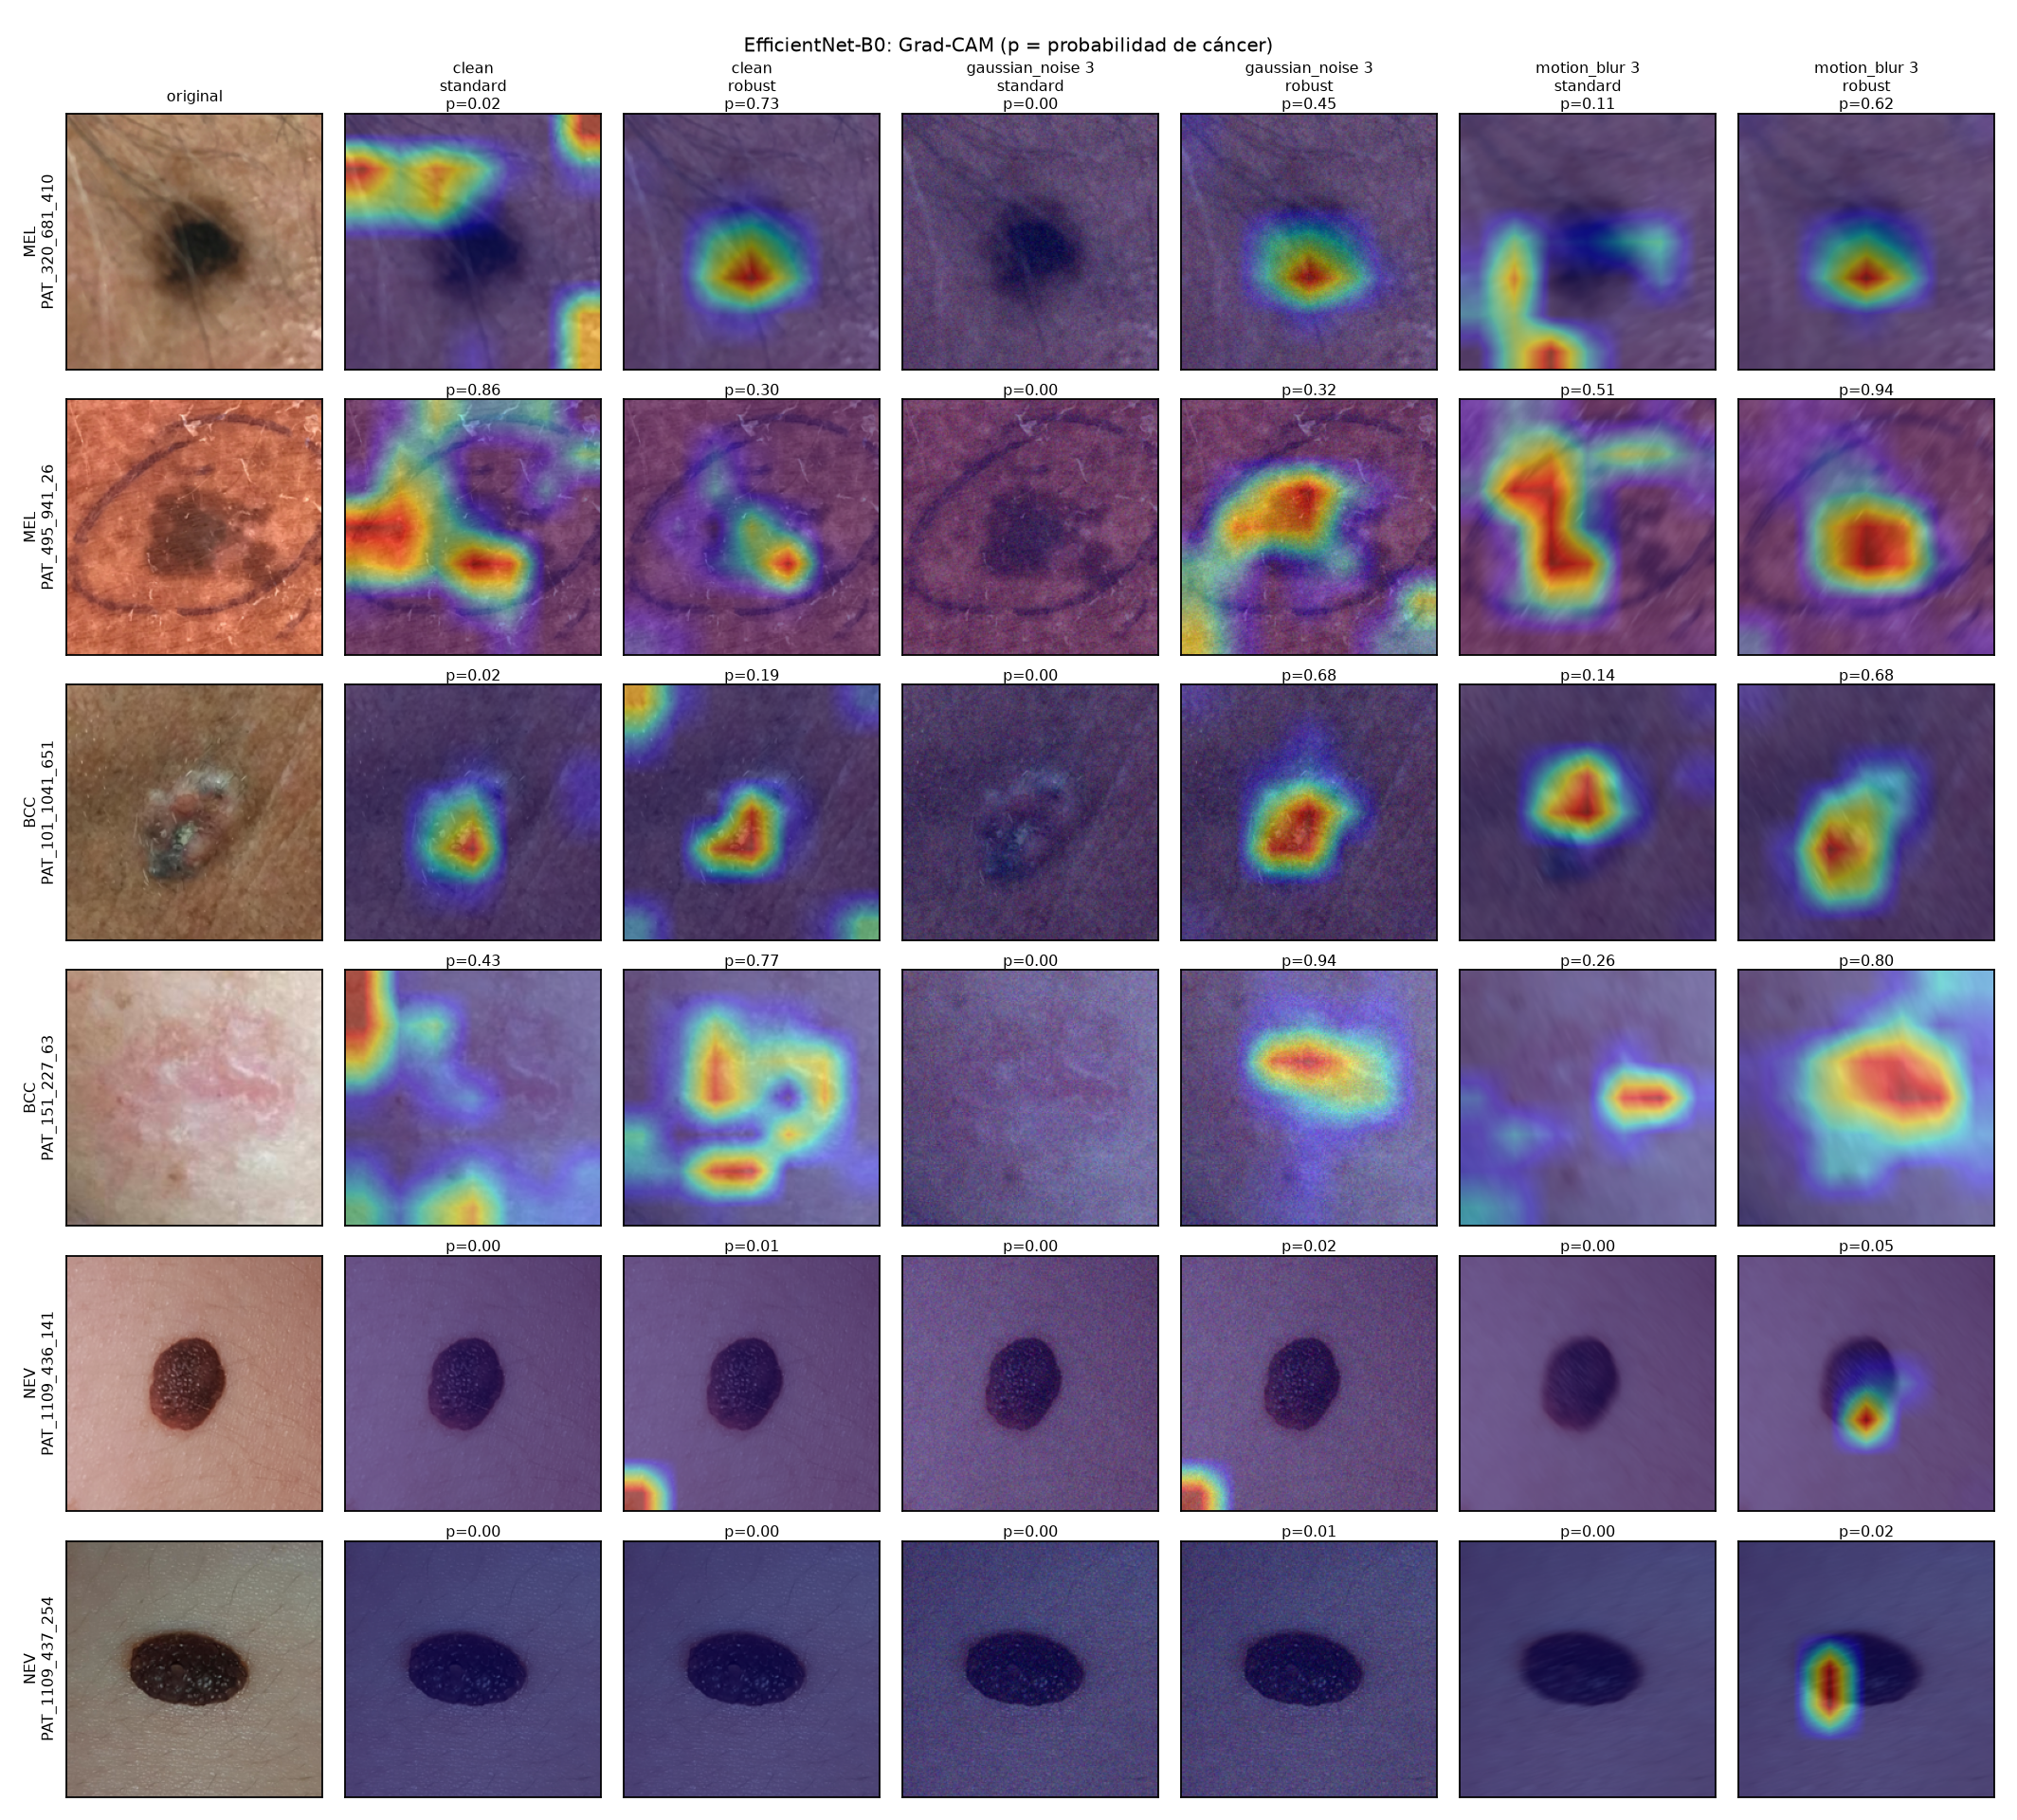
\includegraphics[width=\linewidth]{gradcam_effb0.png}\\(a) EfficientNet-B0, Grad-CAM
\end{minipage}\hfill
\begin{minipage}{0.49\textwidth}\centering
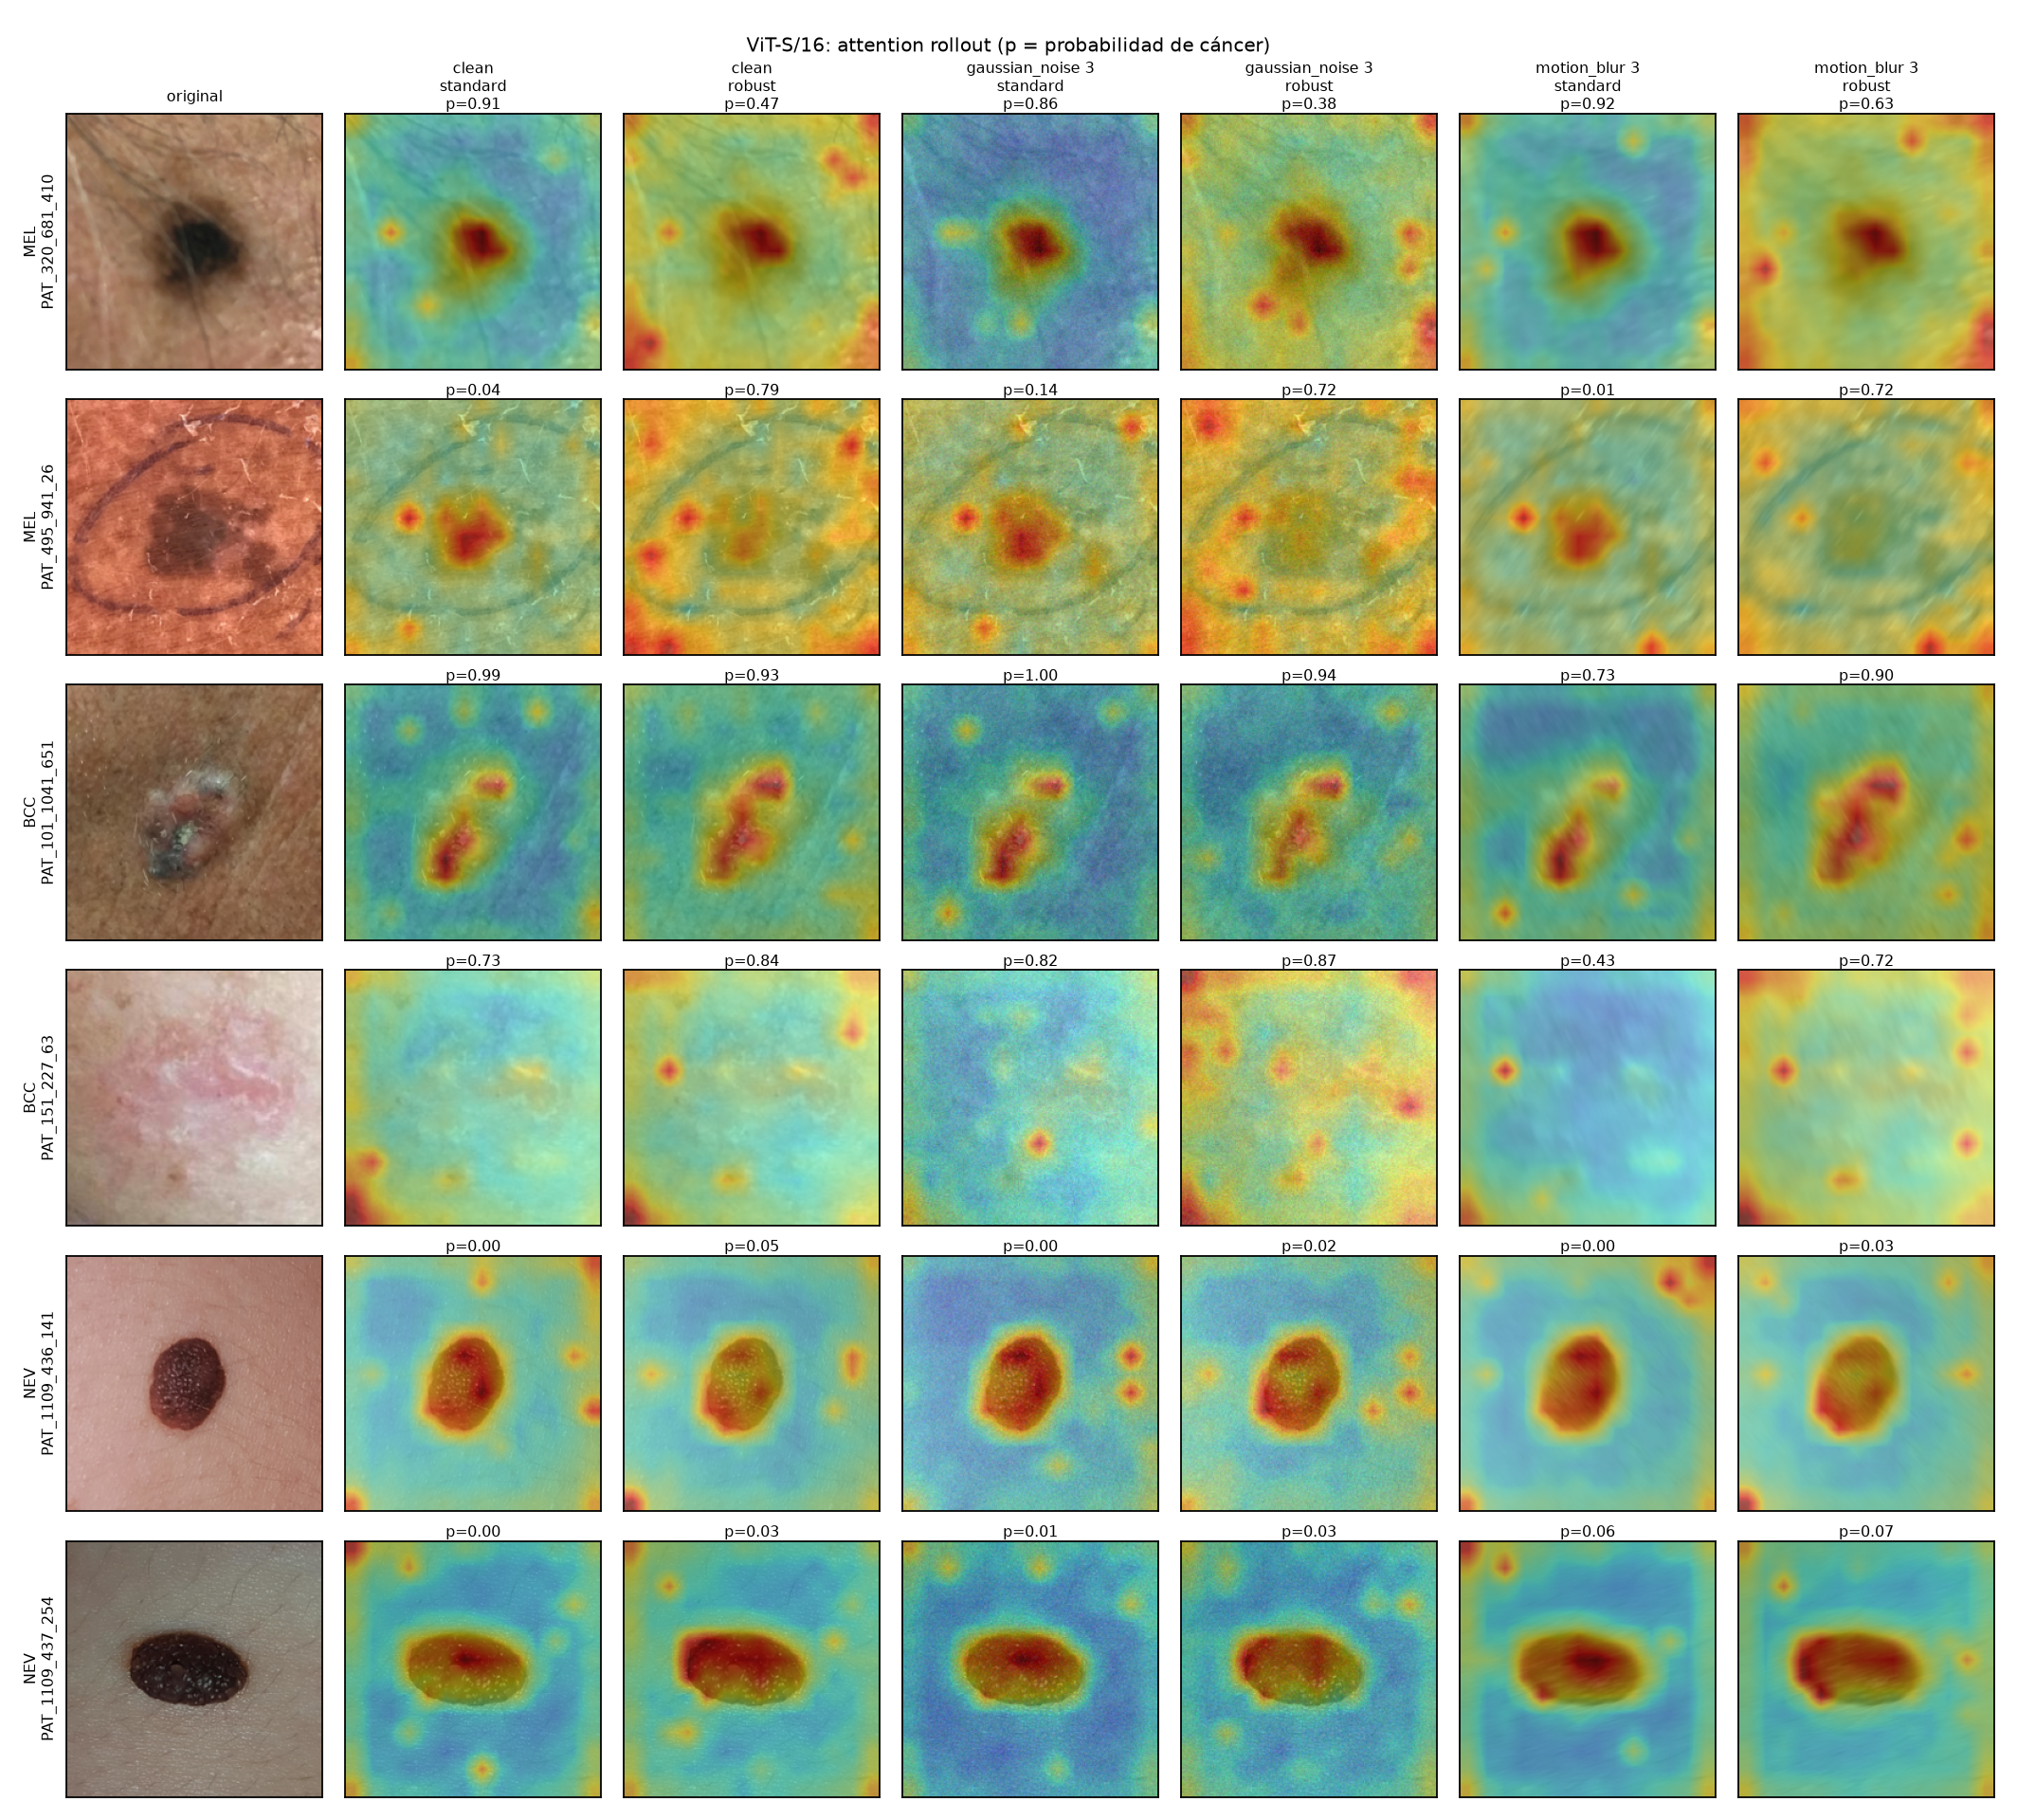
\includegraphics[width=\linewidth]{rollout_vits16.png}\\(b) ViT-S/16, attention rollout
\end{minipage}
\caption{Mapas de evidencia de cáncer en lesiones de test (MEL, BCC, NEV), limpias y con ruido gaussiano o desenfoque de movimiento de severidad 3, para las variantes \texttt{standard} y \texttt{robust}; $p$ es la probabilidad de cáncer.}
\label{fig:maps}
\end{figure*}
\tab{explain_stability}
\begin{figure}[t]
\centering
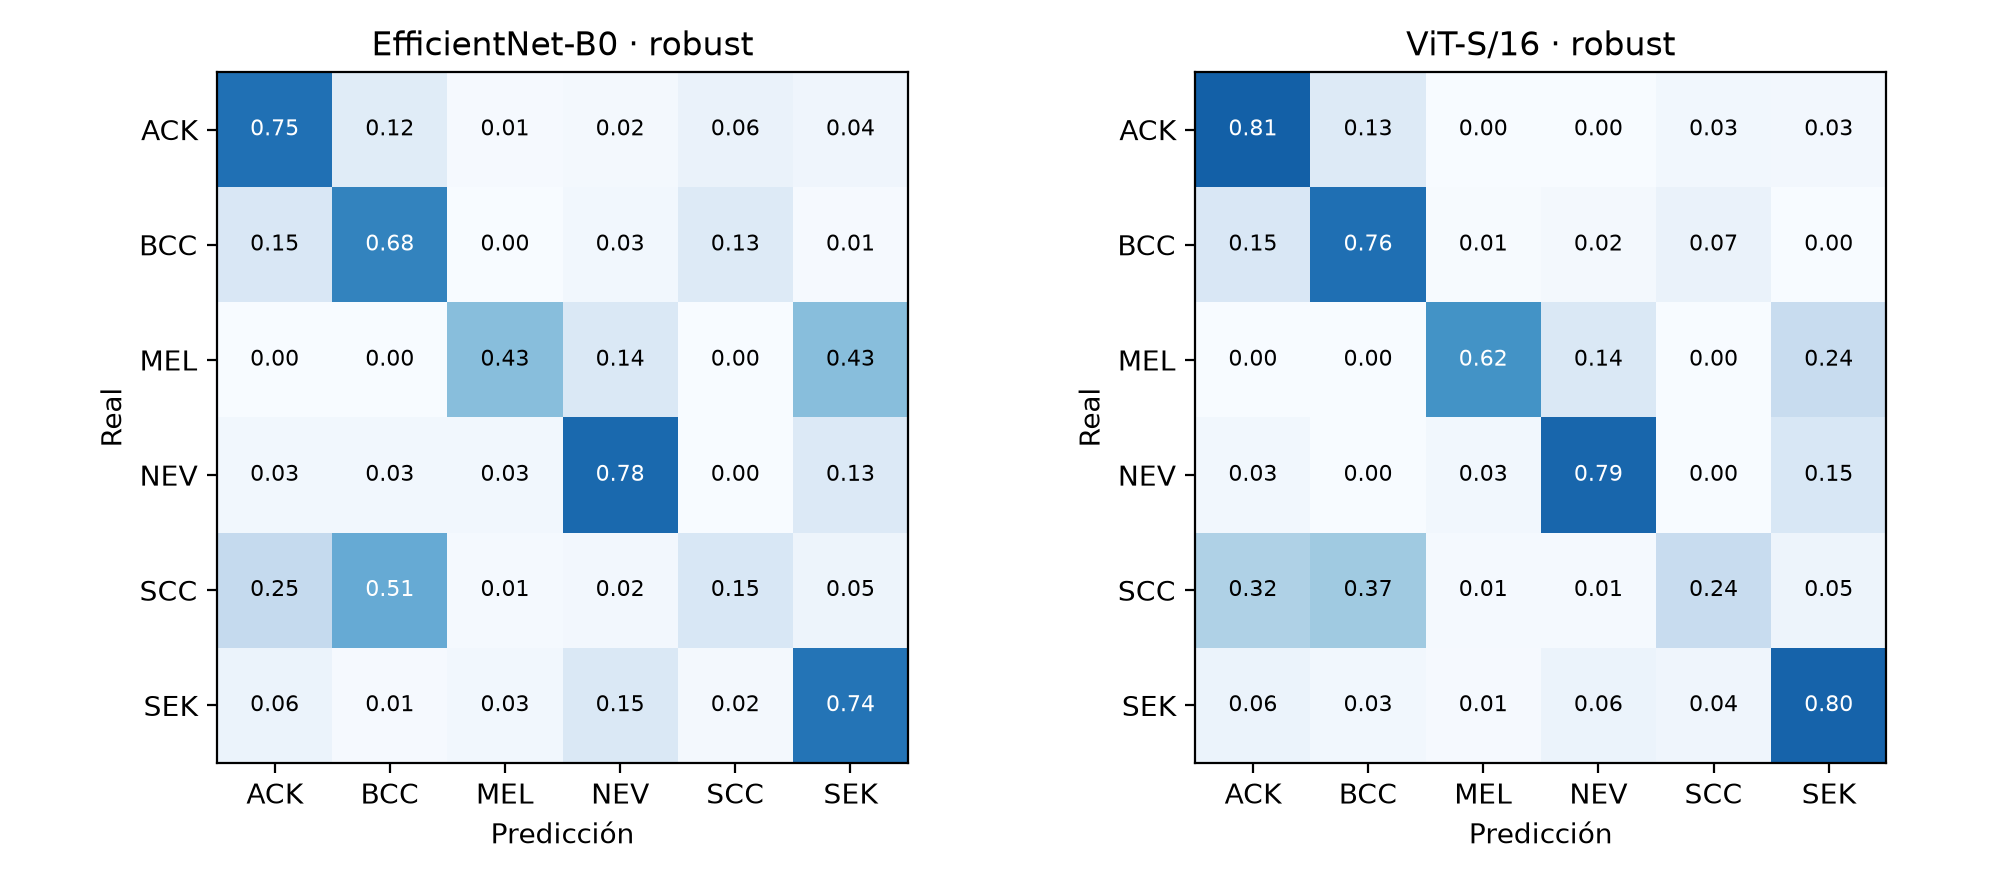
\includegraphics[width=\columnwidth]{confusion_robust.png}
\caption{Matriz de confusión de 6 clases en test limpio de los modelos \texttt{robust}, sumada sobre las 3 semillas y normalizada por fila.}
\label{fig:confusion}
\end{figure}
\tab{subtype}
\tab{bias}
\tab{cost}
\tab{inference}

\subsection{Entrenamiento y métricas}
Usamos AdamW \cite{loshchilov2019} con tasa de aprendizaje $3\times10^{-4}$ para EfficientNet-B0 y $10^{-4}$ para ViT-S/16, decaimiento de pesos 0.05, schedule coseno, lotes de 32 y hasta 30 épocas, con parada temprana de paciencia 7 sobre la AUC cáncer en validación. Cada configuración se entrena con 3 semillas, que cambian la inicialización de la cabeza y el orden de los datos pero no la partición; el modelo HAM se entrena con una semilla y augmentation \texttt{standard}. Los hiperparámetros, la parada temprana y el umbral se eligen solo con validación, y el test se evalúa una vez por corrida.

La métrica principal es la AUC de $\pc$, porque no depende del umbral y es adecuada con clases desbalanceadas; su IC 95\,\% se obtiene por bootstrap de pacientes \cite{efron1993} (1000 remuestreos). Como punto de operación reportamos la especificidad a sensibilidad 90\,\%: el umbral $\tau$ se fija en validación limpia y se aplica sin cambios en test, porque en triaje un cáncer no derivado cuesta más que una derivación de más. La robustez se mide con la caída relativa
\begin{equation}
\Delta_{c,s} = \frac{\mathrm{AUC}_{\mathrm{limpia}} - \mathrm{AUC}_{c,s}}{\mathrm{AUC}_{\mathrm{limpia}}},
\end{equation}
promediada sobre las severidades $s$ de cada corrupción $c$. Para comparar dos condiciones calculamos la diferencia de AUC entre sus medias de semillas, en limpio y como media de las 30 condiciones corruptas, con los mismos remuestreos de pacientes para ambas; un IC que excluye el cero indica una diferencia significativa. Como métricas secundarias reportamos BACC y macro-F1 en 6 clases, que pesan igual todas las clases, la sensibilidad por subtipo con IC exacto de Clopper-Pearson \cite{clopper1934}, y el desempeño por fototipo de Fitzpatrick. Para interpretar los modelos calculamos Grad-CAM \cite{selvaraju2017} de $\log\pc$ sobre la última capa convolucional de EfficientNet-B0 y attention rollout \cite{abnar2020} del token de clase de ViT-S/16; la estabilidad de la explicación es la correlación de Pearson entre el mapa limpio y el mapa con corrupción de severidad 3, promediada sobre los 156 cánceres de test.

Todo está implementado en PyTorch con \texttt{timm} 1.0.30. Las 19 corridas se entrenaron en una GPU NVIDIA T4 de Google Colab con precisión mixta, en 2.73~h en total; la evaluación, la interpretabilidad y la demo corren en una Mac con Apple M4 Pro.

% ---------------------------------------------------------------------------
\section{Resultados}
\label{sec:results}

\subsection{Comparación con la línea base}
La Tabla~\ref{tab:main} compara los modelos con la línea base en test limpio, con la misma partición. Los tres ViT-S/16 alcanzan una AUC de 0.926--0.930 y una especificidad de 0.805--0.830 a la sensibilidad objetivo; EfficientNet-B0 llega a 0.880--0.907, y la línea base a 0.825 con solo 0.445 de especificidad. En limpio, el ViT supera a EfficientNet-B0 con cualquier augmentation (Tabla~\ref{tab:paired}: +0.047 sin augmentation, +0.031 con \texttt{standard} y +0.019 [0.000, 0.038] con \texttt{robust}). La sensibilidad realizada en test (0.87--0.91) queda cerca del 90\,\% fijado en validación, lo que indica que el umbral se transfiere. En 6 clases (Tabla~\ref{tab:main_6class}) el ViT obtiene una BACC de 0.640--0.671, frente a 0.456 de la línea base.

\subsection{Estudio de ablación}
\textbf{Augmentation en la CNN (H1).} La Fig.~\ref{fig:curve} muestra la AUC frente a la severidad y la Tabla~\ref{tab:robustness} la caída relativa por corrupción. Sin augmentation, EfficientNet-B0 pierde el 22.5\,\% de su AUC en las corrupciones vistas y el 20.1\,\% en las no vistas, con caídas del 33--34\,\% bajo desenfoque y ruido gaussianos. Añadir la augmentation \texttt{standard} ayuda sobre todo en las no vistas (10.9\,\%) pero apenas cambia el ruido (33.1\,\%). Con \texttt{robust} la caída baja al 2.7\,\% en las vistas y al 4.8\,\% en las no vistas: el desenfoque de movimiento pasa del 14.1\,\% (\texttt{standard}) al 4.9\,\% y la compresión JPEG del 7.7\,\% al 4.7\,\%. Las diferencias emparejadas (Tabla~\ref{tab:paired}) confirman que \texttt{robust} supera a \texttt{standard} bajo corrupción en +0.128 [0.110, 0.147] sin perder AUC en limpio (+0.009 [$-$0.009, 0.027]). H1 se cumple para la CNN, también en corrupciones no vistas.

\textbf{Arquitectura (H2).} ViT-S/16 sin augmentation pierde solo el 4.2\,\% en ambos grupos de corrupciones, y su peor caso es el desenfoque gaussiano (6.4\,\%), no el ruido. La augmentation \texttt{standard} no cambia su robustez (+0.006 [$-$0.007, 0.020] bajo corrupción), y \texttt{robust} la mejora poco pero de forma significativa (caída del 1.6\,\% y 2.0\,\%; +0.017 [0.005, 0.027] frente a \texttt{standard}). La ventaja del ViT bajo corrupción es grande sin augmentation (+0.198) y con \texttt{standard} (+0.145), y casi desaparece con \texttt{robust} (+0.034 [0.019, 0.050]): la augmentation de adquisición cierra la mayor parte de la brecha de robustez entre arquitecturas.

\textbf{Datos de entrenamiento (H3).} EfficientNet-B0 entrenado en HAM10000 alcanza una AUC de 0.910 en su propia validación, pero de 0.755 [0.694, 0.805] en el test de PAD: 0.143 [0.095, 0.195] menos que el mismo modelo entrenado en PAD, y 0.127 menos bajo corrupción (Tabla~\ref{tab:paired}). Su especificidad cae a 0.376 y su BACC a 0.347. El 63\,\% de las ACK se clasifica como SEK y el 24\,\% como BCC, y la mediana de $\pc$ de las ACK sube de 0.01 a 0.31; el 57\,\% de los melanomas se clasifica como NEV. H3 se cumple, con la salvedad de que este experimento tiene una sola semilla.

\subsection{Interpretabilidad y análisis de errores}
\textbf{Dónde mira el modelo.} La Fig.~\ref{fig:maps} compara los mapas de las variantes \texttt{standard} y \texttt{robust}. EfficientNet-B0 \texttt{standard} pone parte de su evidencia fuera de la lesión, en bordes de piel y marcas de bolígrafo, y bajo ruido gaussiano su mapa se vacía; con \texttt{robust} el mapa se concentra en la lesión y se mantiene con la corrupción. La Tabla~\ref{tab:explain_stability} lo cuantifica: la correlación entre el mapa limpio y el corrupto sube de 0.48 a 0.68 en promedio, y de 0.01 a 0.67 bajo ruido. En el ViT la estabilidad es alta con ambas augmentations (0.78), aunque \texttt{robust} es menos estable bajo vello (0.57 frente a 0.70). Los mapas del ViT muestran artefactos en las esquinas, coherentes con los tokens de norma alta descritos en \cite{darcet2024}.

\textbf{Errores por clase y subtipo.} La matriz de confusión de los modelos \texttt{robust} (Fig.~\ref{fig:confusion}) muestra que SCC se confunde sobre todo con BCC (51\,\% en EfficientNet-B0, 37\,\% en ViT) y con ACK (25\,\% y 32\,\%), y MEL con SEK (43\,\% y 24\,\%) y NEV (14\,\%). Confundir SCC con BCC no afecta al triaje; confundirlo con ACK, una lesión precancerosa, sí. Al umbral de operación (Tabla~\ref{tab:subtype}), BCC (0.90--0.93) domina el resultado binario, porque es el 78\,\% de los cánceres de test; SCC es más difícil (0.79--0.87). Para MEL, con solo 7 imágenes de 5 lesiones, el ViT con \texttt{standard} o \texttt{robust} detecta 0.71--0.76 y EfficientNet-B0 0.43--0.57, pero los IC exactos son muy amplios (p.\,ej. [0.29, 0.96]). Una lesión (2 fotos de un mismo paciente) no se deriva con casi ningún modelo. La línea base detecta los 7 melanomas porque su umbral es mucho más bajo, a costa de derivar a más de la mitad de los no cánceres.

\textbf{Fototipo.} La Tabla~\ref{tab:bias} separa el test por fototipo de Fitzpatrick. Todos los modelos rinden peor en los fototipos I--II (AUC 0.77--0.82) que en III--VI (0.87--0.97), sobre todo por una especificidad más baja (0.41--0.58). La comparación es frágil: el grupo III--VI tiene solo 15 no cánceres, el fototipo falta en 118 imágenes (todas de no cáncer), y los no cánceres de I--II son ACK en un 80\,\% (32 de 40) frente a un 67\,\% en III--VI, donde además hay 5 NEV, más fáciles de descartar. Los fototipos IV--VI son escasos (12 imágenes de test), así que el grupo III--VI es sobre todo fototipo III, y estos resultados no permiten afirmar que el modelo sea equitativo en piel oscura \cite{daneshjou2022}.

\subsection{Costo computacional}
Las 19 corridas, incluidas las de las configuraciones descartadas, suman 2.73~h de GPU T4 (Tabla~\ref{tab:cost}), unos 0.19~kWh con los 70~W de TDP de la T4. Una corrida \texttt{robust} cuesta unas 2.1--2.3 veces más que una \texttt{standard} (12--14 frente a 6~min), porque las corrupciones se aplican en CPU. En inferencia (Tabla~\ref{tab:inference}), ambos modelos clasifican una imagen en menos de 10~ms en la GPU de la Mac. En CPU, ViT-S/16 tarda 20~ms y EfficientNet-B0 unos 275~ms, pese a tener 5 veces menos parámetros; atribuimos esta diferencia a que las convoluciones depthwise están poco optimizadas en la CPU arm64 de esta versión de PyTorch, no a la arquitectura.

% ---------------------------------------------------------------------------
\section{Discusión}
\label{sec:discussion}

\textbf{Por qué funciona.} Las corrupciones que más dañan a la CNN, el ruido y el desenfoque, alteran la textura de alta frecuencia en la que se apoyan las CNN entrenadas con ImageNet. La augmentation \texttt{standard} solo cambia la geometría y no toca esa textura, mientras que \texttt{robust} obliga al modelo a basarse en rasgos que sobreviven a la degradación; Grad-CAM lo muestra como una evidencia más concentrada en la lesión y más estable. Que la mejora alcance también al desenfoque de movimiento y a la compresión JPEG, nunca vistos en entrenamiento, sugiere que el modelo aprende una invarianza más general y no solo las cuatro corrupciones concretas. El ViT, que integra información global desde la primera capa, ya es robusto sin augmentation, en línea con \cite{bhojanapalli2021}; para él la augmentation de adquisición aporta poco, pero tampoco cuesta AUC en limpio.

\textbf{Comparación con lo publicado.} Nuestra BACC en 6 clases (0.67) está por debajo del $\approx$0.77 de \cite{pacheco2021metablock}, que además usa los metadatos clínicos del paciente y validación cruzada en lugar de una partición fija por paciente, así que la comparación es solo orientativa. Nuestros resultados coinciden con \cite{maron2021,young2021} en que las CNN estándar son frágiles ante degradaciones, y muestran que esa fragilidad se corrige en gran parte entrenando con degradaciones realistas. El experimento HAM$\to$PAD confirma que un buen resultado con imágenes dermatoscópicas no se transfiere a fotos clínicas.

\textbf{Limitaciones.} PAD-UFES-20 tiene 52 melanomas, 7 en test, así que la sensibilidad para MEL es solo descriptiva. ACK es precancerosa y se cuenta como no cáncer, siguiendo la convención del conjunto, y el mapeo de \texttt{akiec} de HAM10000 a SCC es ambiguo. Los datos vienen de un solo programa en Brasil, con mayoría de fototipos I--III y fotos tomadas por profesionales, lo que limita la validez externa. Las corrupciones sintéticas aproximan, pero no reproducen, las degradaciones de una foto real, y no cubren el encuadre, la distancia o la sombra del teléfono. Usamos 3 semillas (1 para HAM) y no hicimos búsqueda de hiperparámetros.

\textbf{Sesgos, riesgos e impacto.} El peor desempeño en fototipos claros y la escasez de fototipos oscuros impiden garantizar un comportamiento equitativo; un despliegue requeriría datos de la población objetivo. El modelo es una herramienta de apoyo al triaje, no un diagnóstico, y no ha sido validado de forma prospectiva: su umbral está fijado para no perder más del 10\,\% de los cánceres, lo que implica derivar a parte de las lesiones benignas, y un falso negativo podría retrasar un diagnóstico si se usara sin supervisión médica. Las fotos de piel son datos de salud identificables; por eso la demo web que acompaña al trabajo corre solo en local, no almacena las imágenes y muestra un aviso explícito de que no es un dispositivo médico. Bien validado, un triaje así podría acortar la espera de dermatología en zonas con pocos especialistas.

% ---------------------------------------------------------------------------
\section{Conclusiones}
\label{sec:conclusions}

La calidad de la foto es una fuente de error tan importante como la arquitectura: una CNN entrenada de forma convencional puede perder más de un tercio de su AUC con ruido o desenfoque moderados, mientras que la misma red entrenada con degradaciones simuladas apenas se ve afectada, incluso con degradaciones que no vio. El Vision Transformer es más preciso y robusto de partida, pero la augmentation de adquisición reduce su ventaja sobre la CNN a 0.03 de AUC bajo corrupción, de modo que la elección de arquitectura pesa menos que el entrenamiento cuando el costo de cómputo importa.

Como trabajo futuro proponemos validar el modelo con fotos degradadas reales tomadas en consulta, ampliar los datos con más melanomas y fototipos IV--VI, incorporar los metadatos clínicos de PAD-UFES-20 al modelo robusto, y estimar la incertidumbre de la predicción para rechazar fotos de calidad insuficiente.

% ---------------------------------------------------------------------------
\section*{Contribuciones}

\begin{center}
\begin{tabular}{>{\raggedright\arraybackslash}p{0.5\columnwidth}>{\raggedright\arraybackslash}p{0.4\columnwidth}}
\toprule
Integrante & Tareas en las que participó \\
\midrule
Juan Burgos Choquehuanca & -- \\
David Roberto Paredes Abanto & -- \\
Carlos Adrian Salguero Torres & -- \\
Huber Angel Ramirez Quispe & -- \\
\bottomrule
\end{tabular}
\end{center}

% Sección comentada por ahora.
% \section*{Disponibilidad de código y uso de herramientas de IA}
% El código, las particiones, las predicciones y los comandos para regenerar cada tabla y figura están en \url{https://github.com/hramirezq/melanoma-detection}; el enlace a los pesos se publica en el README del repositorio. Se usó Claude Code (Anthropic) como asistente de programación (implementación y depuración del código) y de redacción. Todo el código y el texto fueron revisados por los autores, y cada número del artículo proviene de los scripts del repositorio.

\bibliographystyle{IEEEtran}
\bibliography{refs}

\end{document}
